\chapter{Guía de uso}
\label{Appendix:guiaUsuario}
En este apéndice se realizará una guía de uso, utilizando capturas de pantalla para explicar todas las funcionalidades tanto desde el punto de vista del usuario como del profesional, el objetivo es que se pueda entender como utilizar la aplicación y qué funcionalidades tiene. Algunas cosas a tener en cuenta sobre esta guía: 
\begin{itemize}
    \item Las capturas están hechas con la aplicación en inglés, como originalmente se programó.
    \item En la sección \ref{sec:guiaProf} solo se han añadido explicaciones sobre las funcionalidades que difieren respecto a los usuarios, las comunes han sido incluidas en la sección de guía de usuario (\ref{sec:guiaUser}).
\end{itemize}

\newpage
\section{Guía de usuario}
\label{sec:guiaUser}
\subsection{Inicio de sesión, registro, y localización}
\begin{figure}[h]
	\centering
	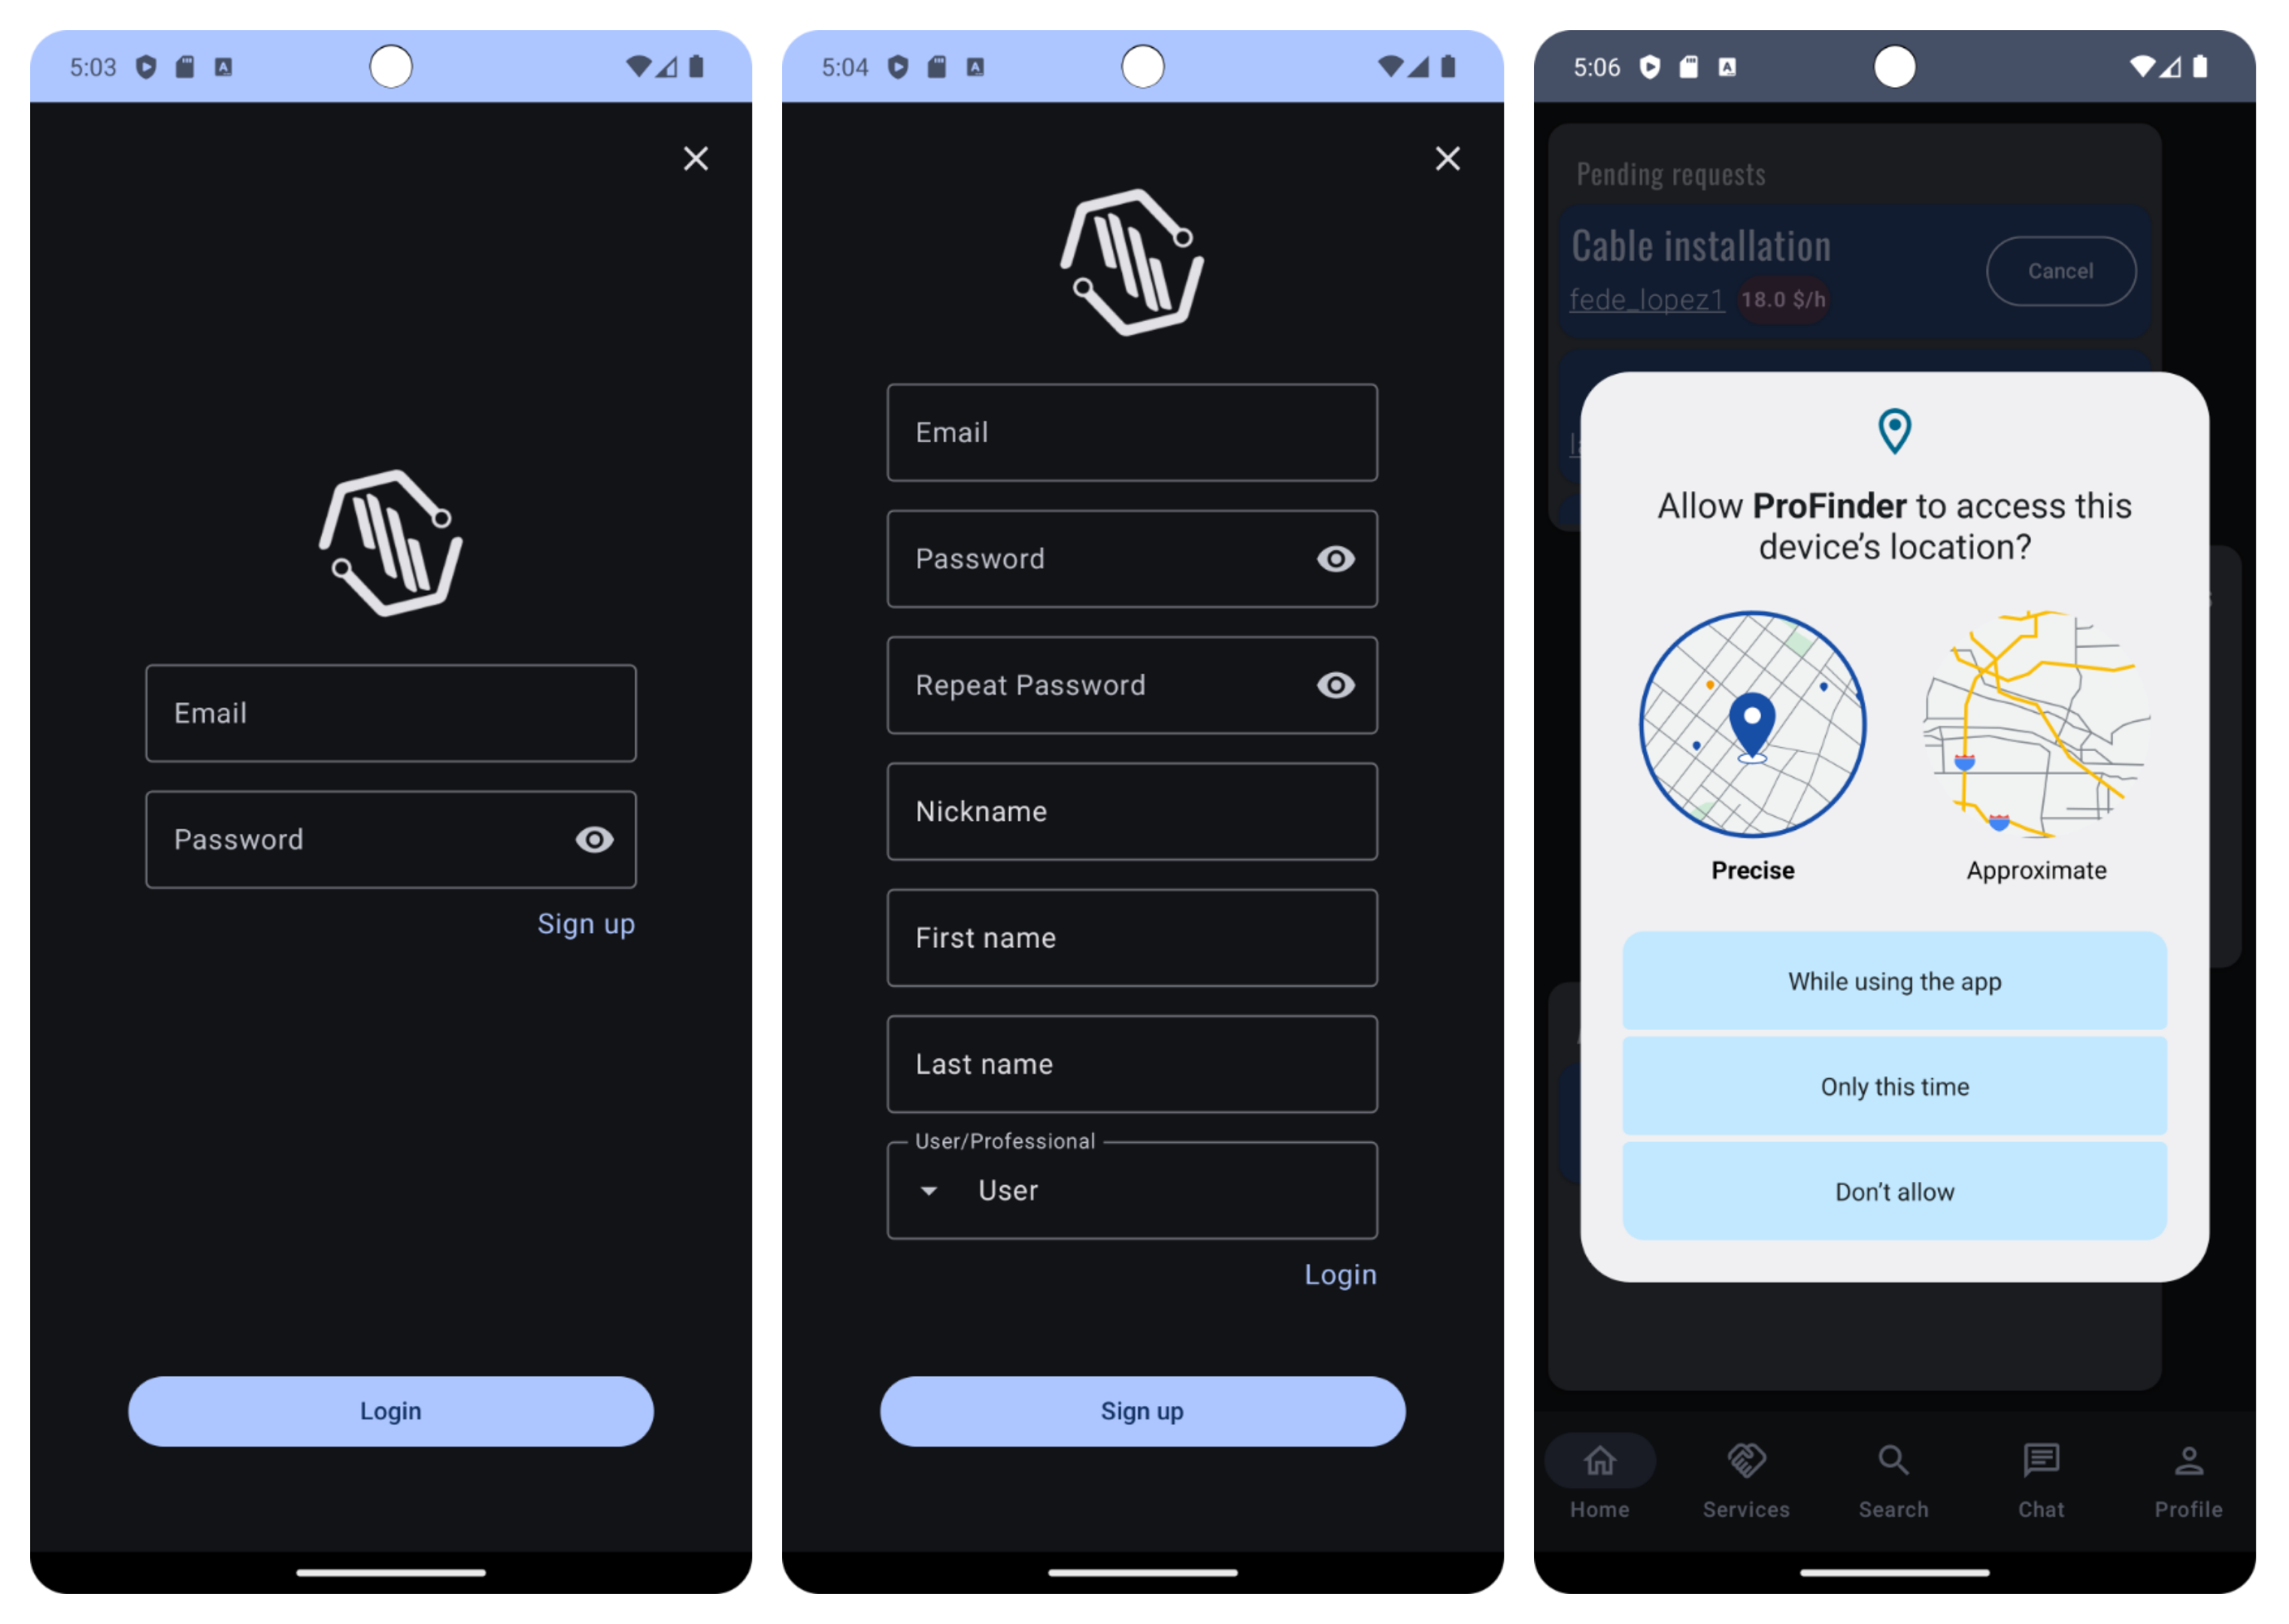
\includegraphics[width = 1\textwidth]{Imagenes/capturasApp/login_signup_local.png}
	\caption{Login Screen, Sign up Screen, permiso de localización}
	\label{fig:capApp1}
\end{figure}
Al entrar en la aplicación, la primera pantalla despues de la pantalla \textit{splash} con el logo de la aplicación que se le mostrará al usuario será la de inicio de sesión -primera captura, figura \ref{fig:capApp1}- (en caso de que el usuario haya iniciado sesión previamente y se haya guardado la misma la primera pantalla que aparecerá será directamente la \textit{home} de la aplicación). En ella el usuario rellenará los campos pertinentes con su correo y contraseña en caso de que tenga una cuenta creada para poder usar la aplicación.

En caso de que el usuario no tenga cuenta creada, pulsando el botón de ‘Sign up’ se le mostrará la pantalla de registro -segunda captura, figura \ref{fig:capApp1}- en la que podrá crear su cuenta.

Al iniciar sesión de forma exitosa, a no ser que ya se haya guardado una preferencia de uso de localización para la aplicación, se solicitarán los permisos para usarla -tercera captura, figura \ref{fig:capApp1}-, ya que esta es necesaria para la funcionalidad de mapa.
\newpage
\subsection{Pantalla de Home, valoración de profesionales y Pantalla de servicios (lista)}
\begin{figure}[h]
	\centering
	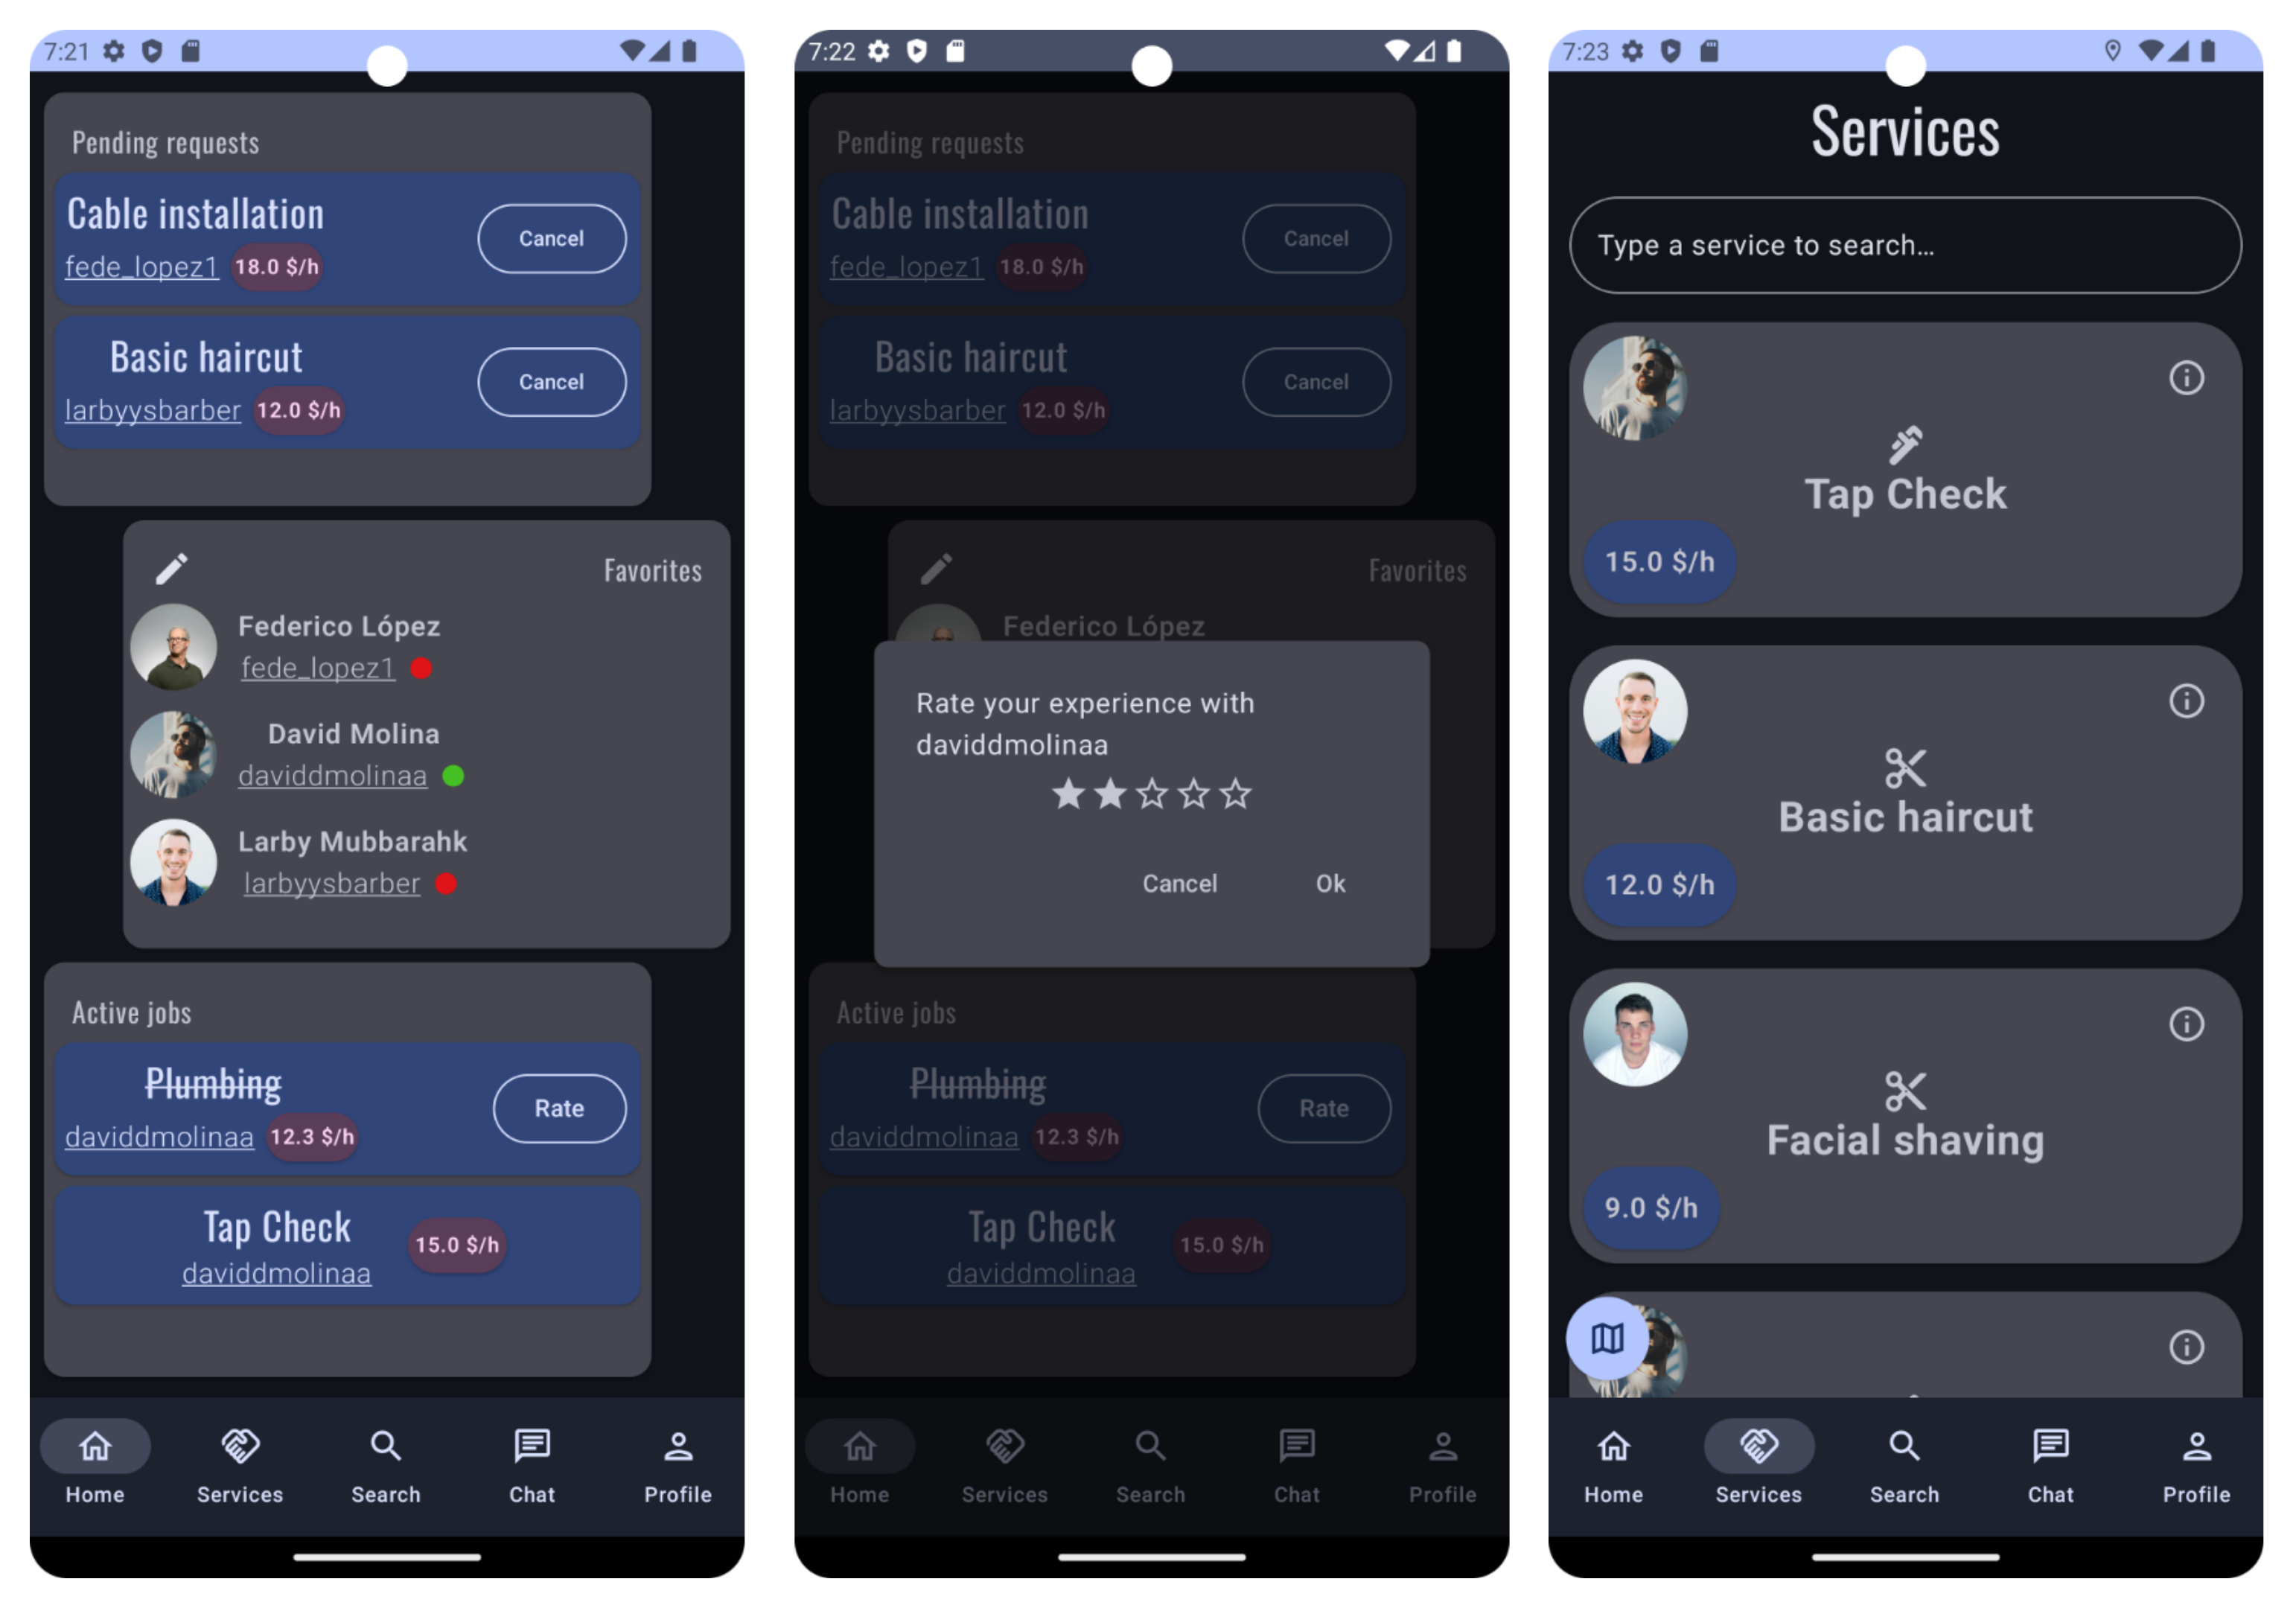
\includegraphics[width = 1\textwidth]{Imagenes/capturasApp/home_rate_services.png}
	\caption{Home Screen, Valorar profesional, Services Screen}
	\label{fig:capApp2}
\end{figure}

La pantalla de \textit{Home} es la principal de la aplicación -captura 1, figura \ref{fig:capApp2}-, en ella, los usuarios podrán ver las solicitudes de servicio que han realizado (también podrán cancelar solicitudes), su lista de favoritos (que también podrán modificar) y los trabajos activos, en caso de que alguno de ellos haya terminado por parte del profesional, saldrá un botón adicional; al pulsarlo podrá valorar el trabajo del profesional -captura 2, figura \ref{fig:capApp2}-.

La siguiente panatalla por la que se podrá navegar usando la \textit{bottom bar} será la pantalla de servicios, esta se divide en distintas partes, la primera y principal será la lista de servicios disponibles -captura 3 \ref{fig:capApp2}- que muestra un resumen de cada servicio (precio, nombre y foto del profesional), se podrán filtrar los servicios por nombre.
\newpage
\subsection{Detalles de servicio, pantalla de servicios (mapa), y pantalla de búsqueda}
\begin{figure}[h]
	\centering
	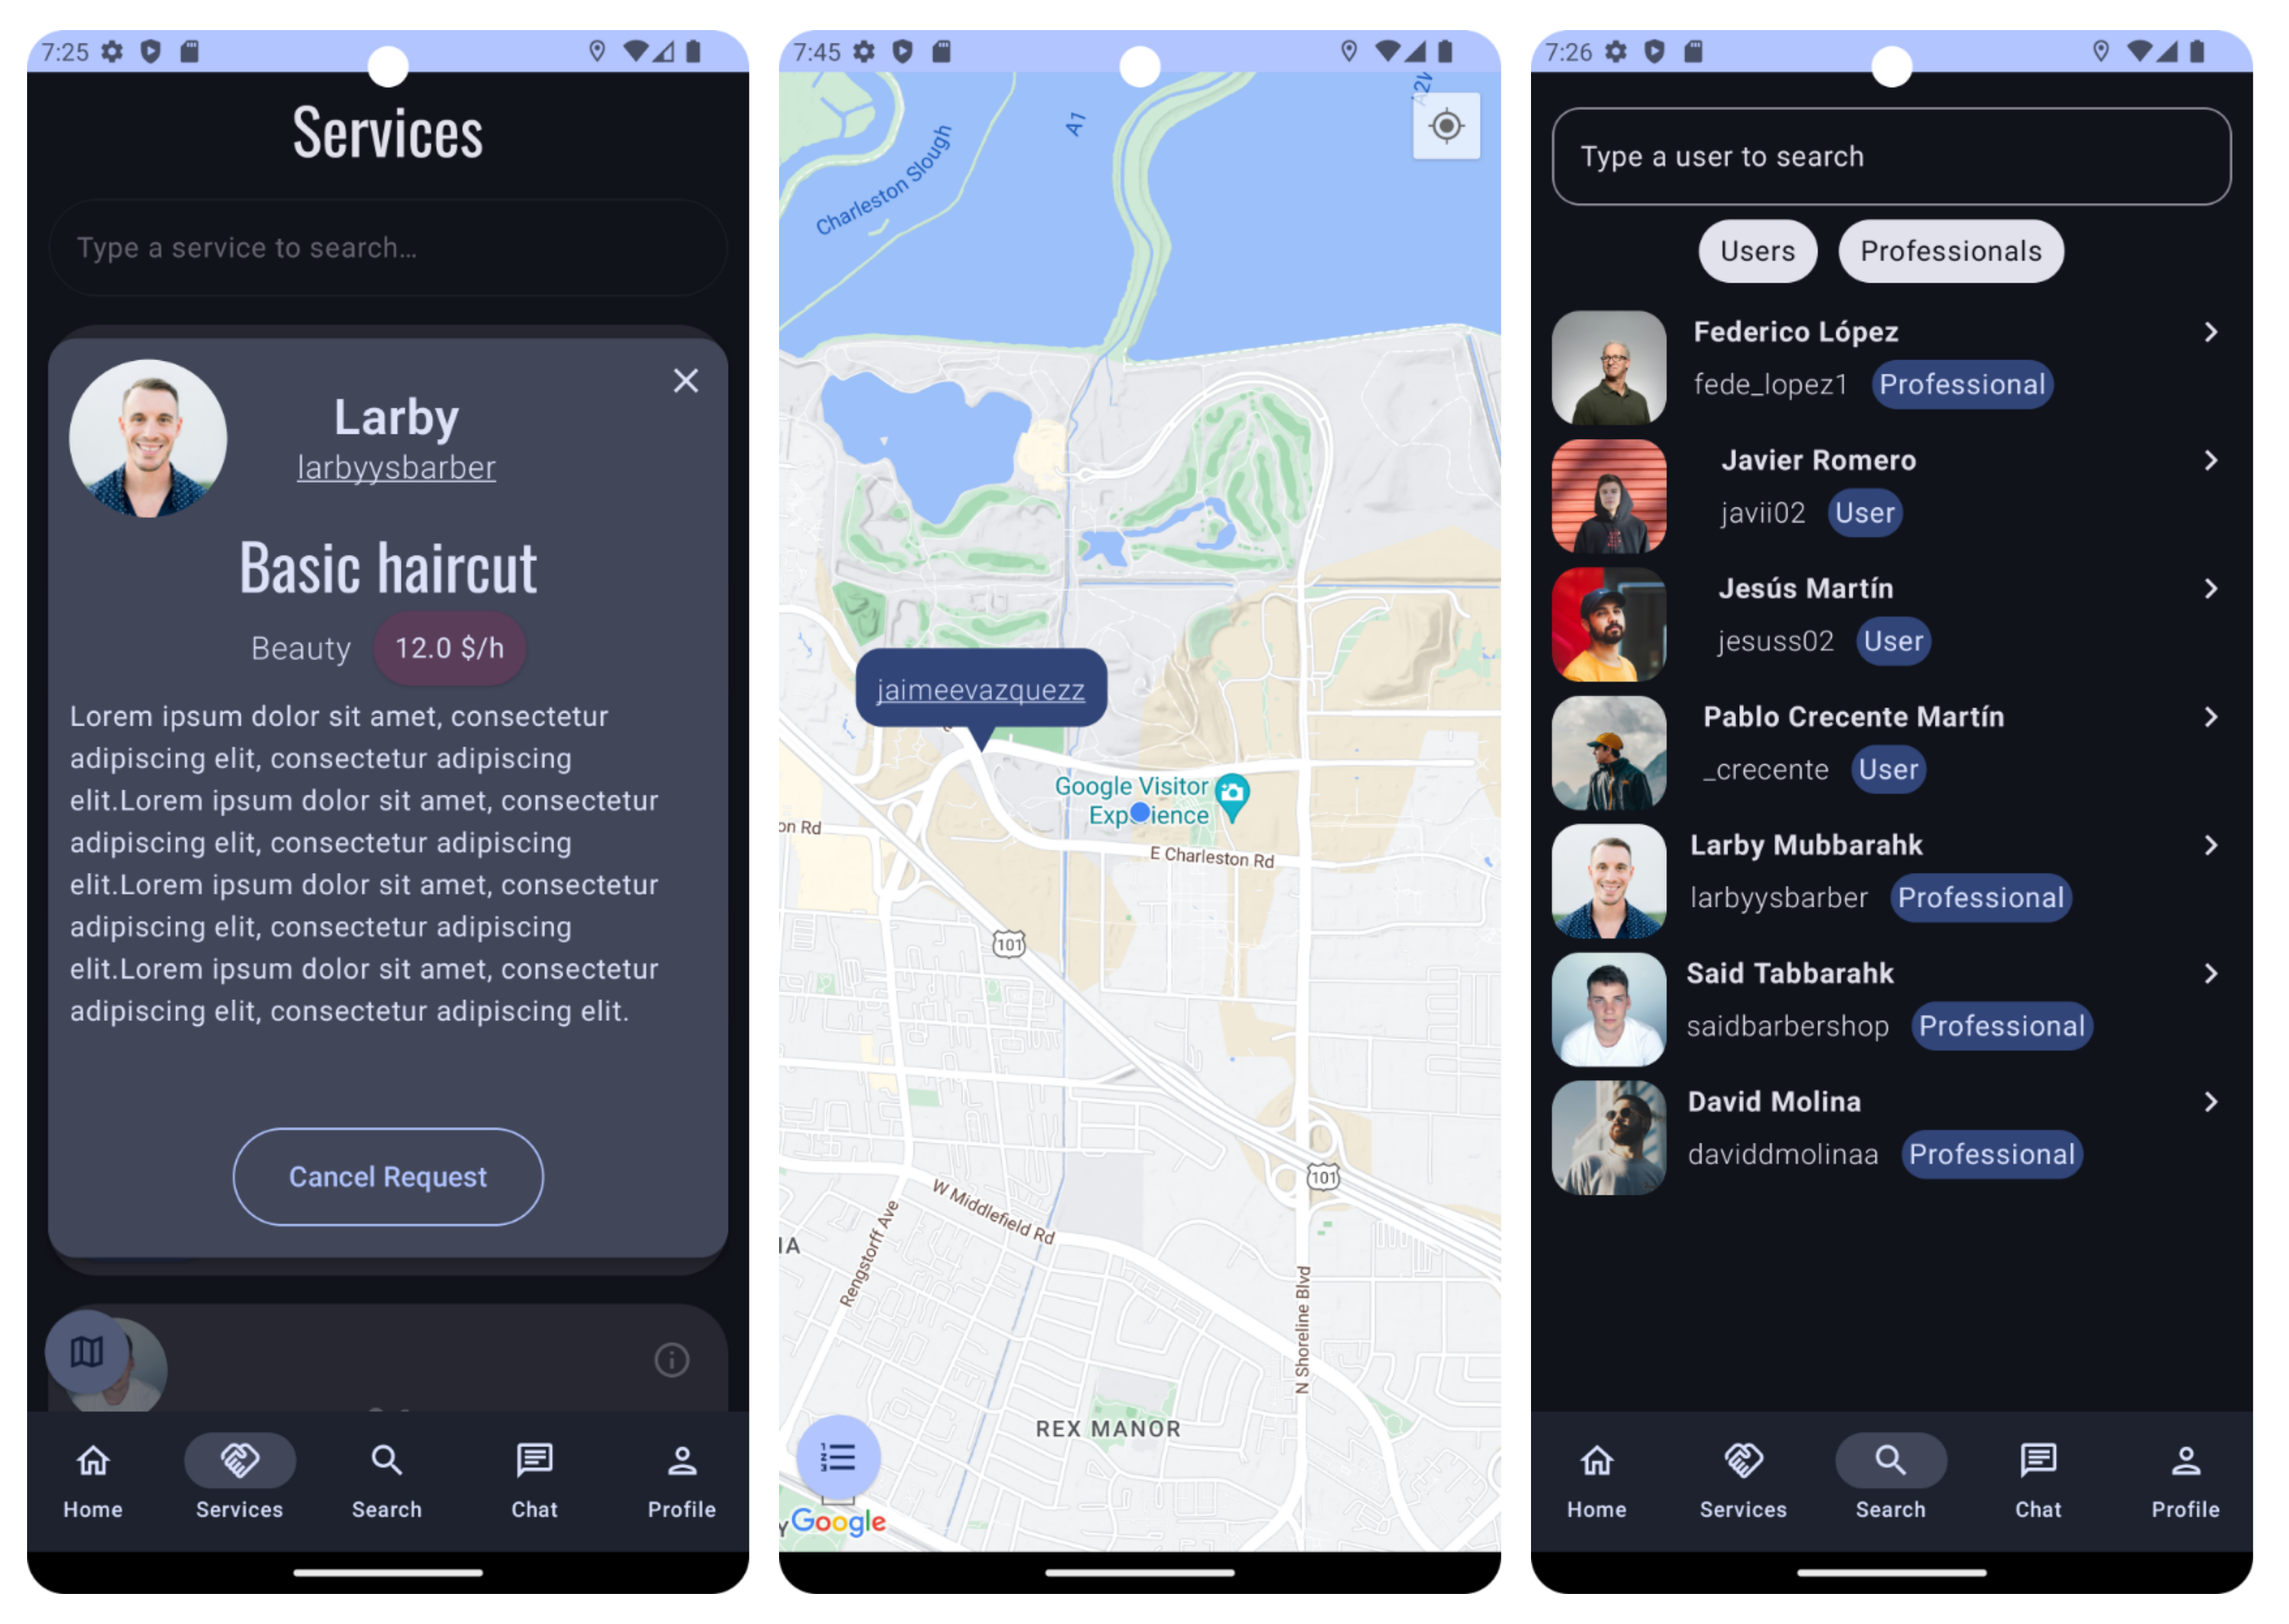
\includegraphics[width = 1\textwidth]{Imagenes/capturasApp/detail_map_search.png}
	\caption{Service Details, Map Screen, Search Screen}
	\label{fig:capApp3}
\end{figure}

En caso de que se quieran tener más detalles de un servicio o solicitarlo se podrá pulsar el icono de información -captura 1, figura \ref{fig:capApp3}-.

Al pulsar en el botón de abajo a la izquierda, encima de la \textit{bottom bar}, se cambiará a la vista de mapa -captura 2, figura \ref{fig:capApp3}-, en la que aparecerán todos los profesionales en el mapa con su última ubicación conocida. Al pulsar en cualquiera de ellos se podrá ver su perfil y servicios activos.

La siguiente pantalla siguiendo el orden de la \textit{bottom bar} será la de búsqueda -captura 3, figura \ref{fig:capApp3}- en ella se podrá buscar cualquier usuario de la aplicación, así como filtrar por usuario/profesional y por nombre de usuario, nombre o apellido. Al pulsar en cualquier item de la lista se abrirá el perfil del actor seleccionado.
\newpage
\subsection{Pantalla para ver otro perfil, chats recientes y chat individual}
\begin{figure}[h]
	\centering
	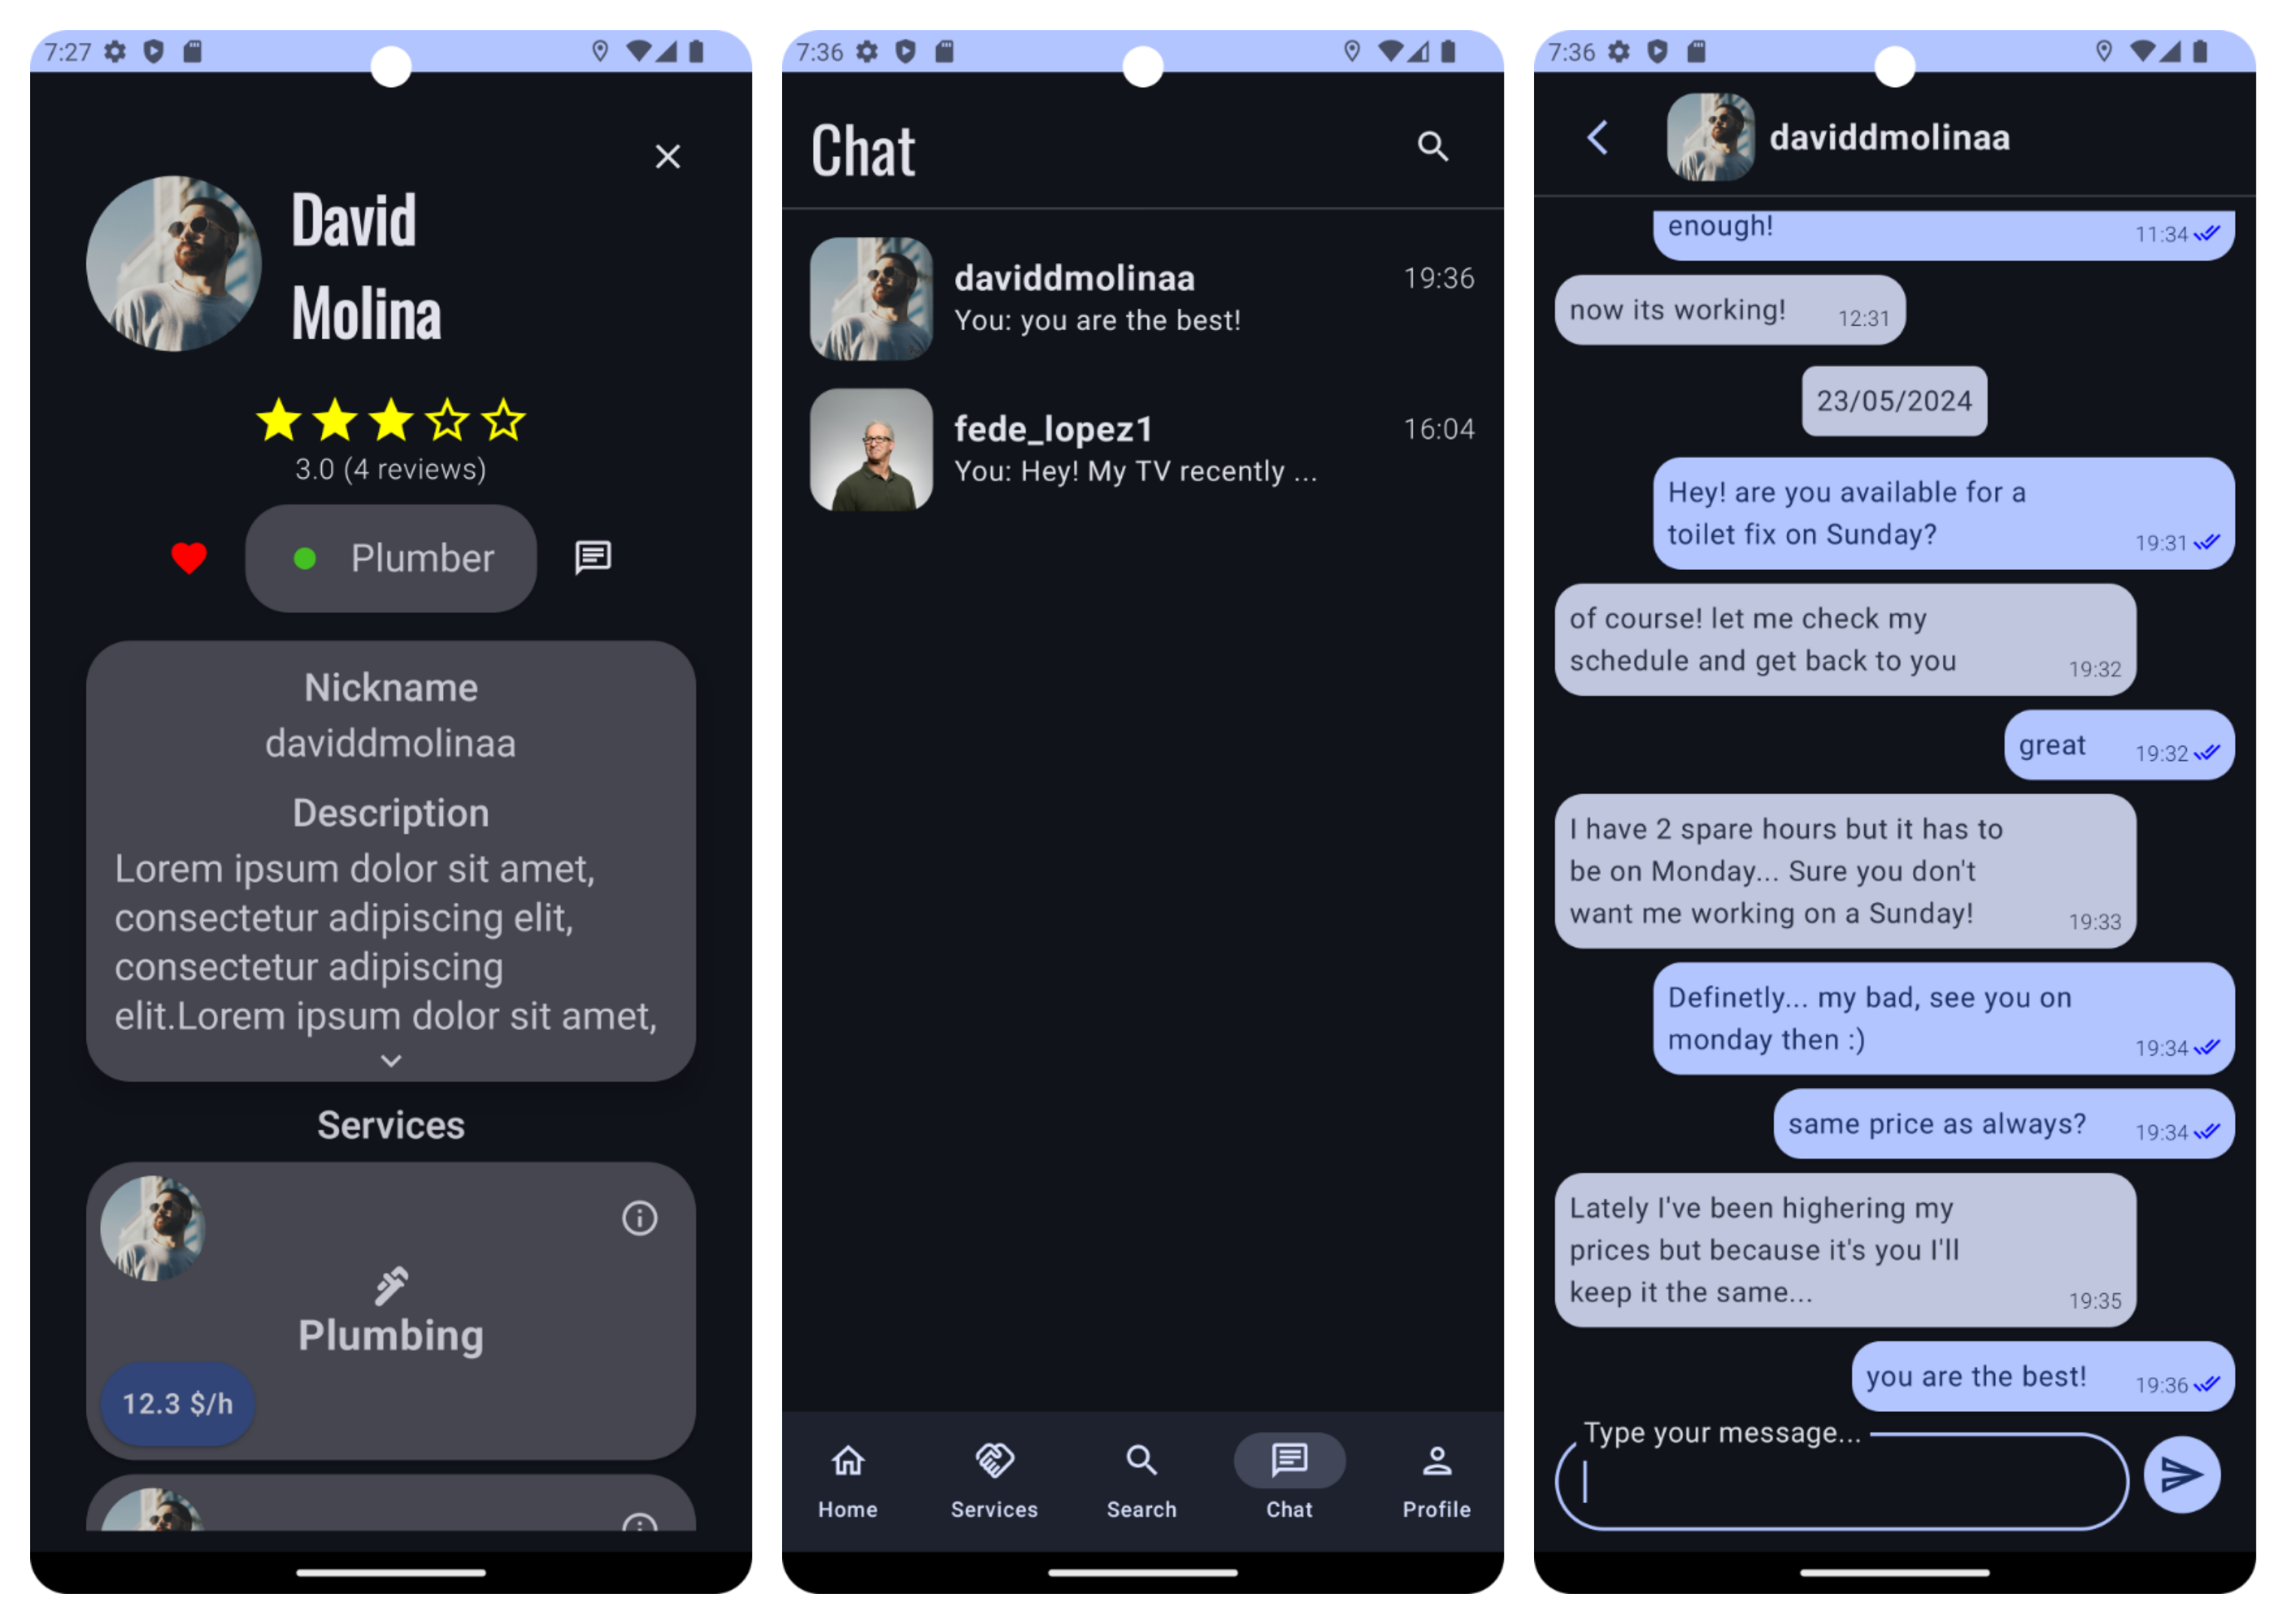
\includegraphics[width = 1\textwidth]{Imagenes/capturasApp/seeProfile_recent_chat.png}
	\caption{View profile Screen, Recent chats Screen, Individual chat Screen}
	\label{fig:capApp4}
\end{figure}

En diversas partes de la aplicación, se podrá pulsar en el  nombre de usuario para ver su perfil, este lleva a la pantalla de  vista de perfil -captura 1, figura \ref{fig:capApp4}- en la que se podrán ver todos los datos relevantes del actor seleccionado como nombre completo, foto de perfil, media y número de \textit{reviews}, estado y profesión (en caso de profesional), nombre de usuario y descripción. También se podrán ver y solicitar los servicios activos en caso de profesional, así como añadir/quitar de la lista de favoritos o abrir el chat individual con ese actor. 

La siguiente sección es la funcionalidad de chat, cuarto botón de la \textit{bottom bar}. En primer lugar, se mostrará una lista con los chats recientes -captura 2, figura \ref{fig:capApp4}- cada una contendrá algunos aspectos acerca de cada chat como el nombre de usuario, foto de perfil del otro participante en el chat, último mensaje y hora del mismo. En esta pantalla se podrá buscar el chat con un usuario específico. Pulsando en un chat de la lista de recientes se accede a la pantalla de chat individual -captura 3, figura \ref{fig:capApp4}-, en la que se podrá mantener una conversación a través de mensajes en tiempo real con la otra persona, así como ver mensajes pasados.
\newpage
\subsection{Pantalla de perfil, modo claro y editar perfil}
\begin{figure}[h]
	\centering
	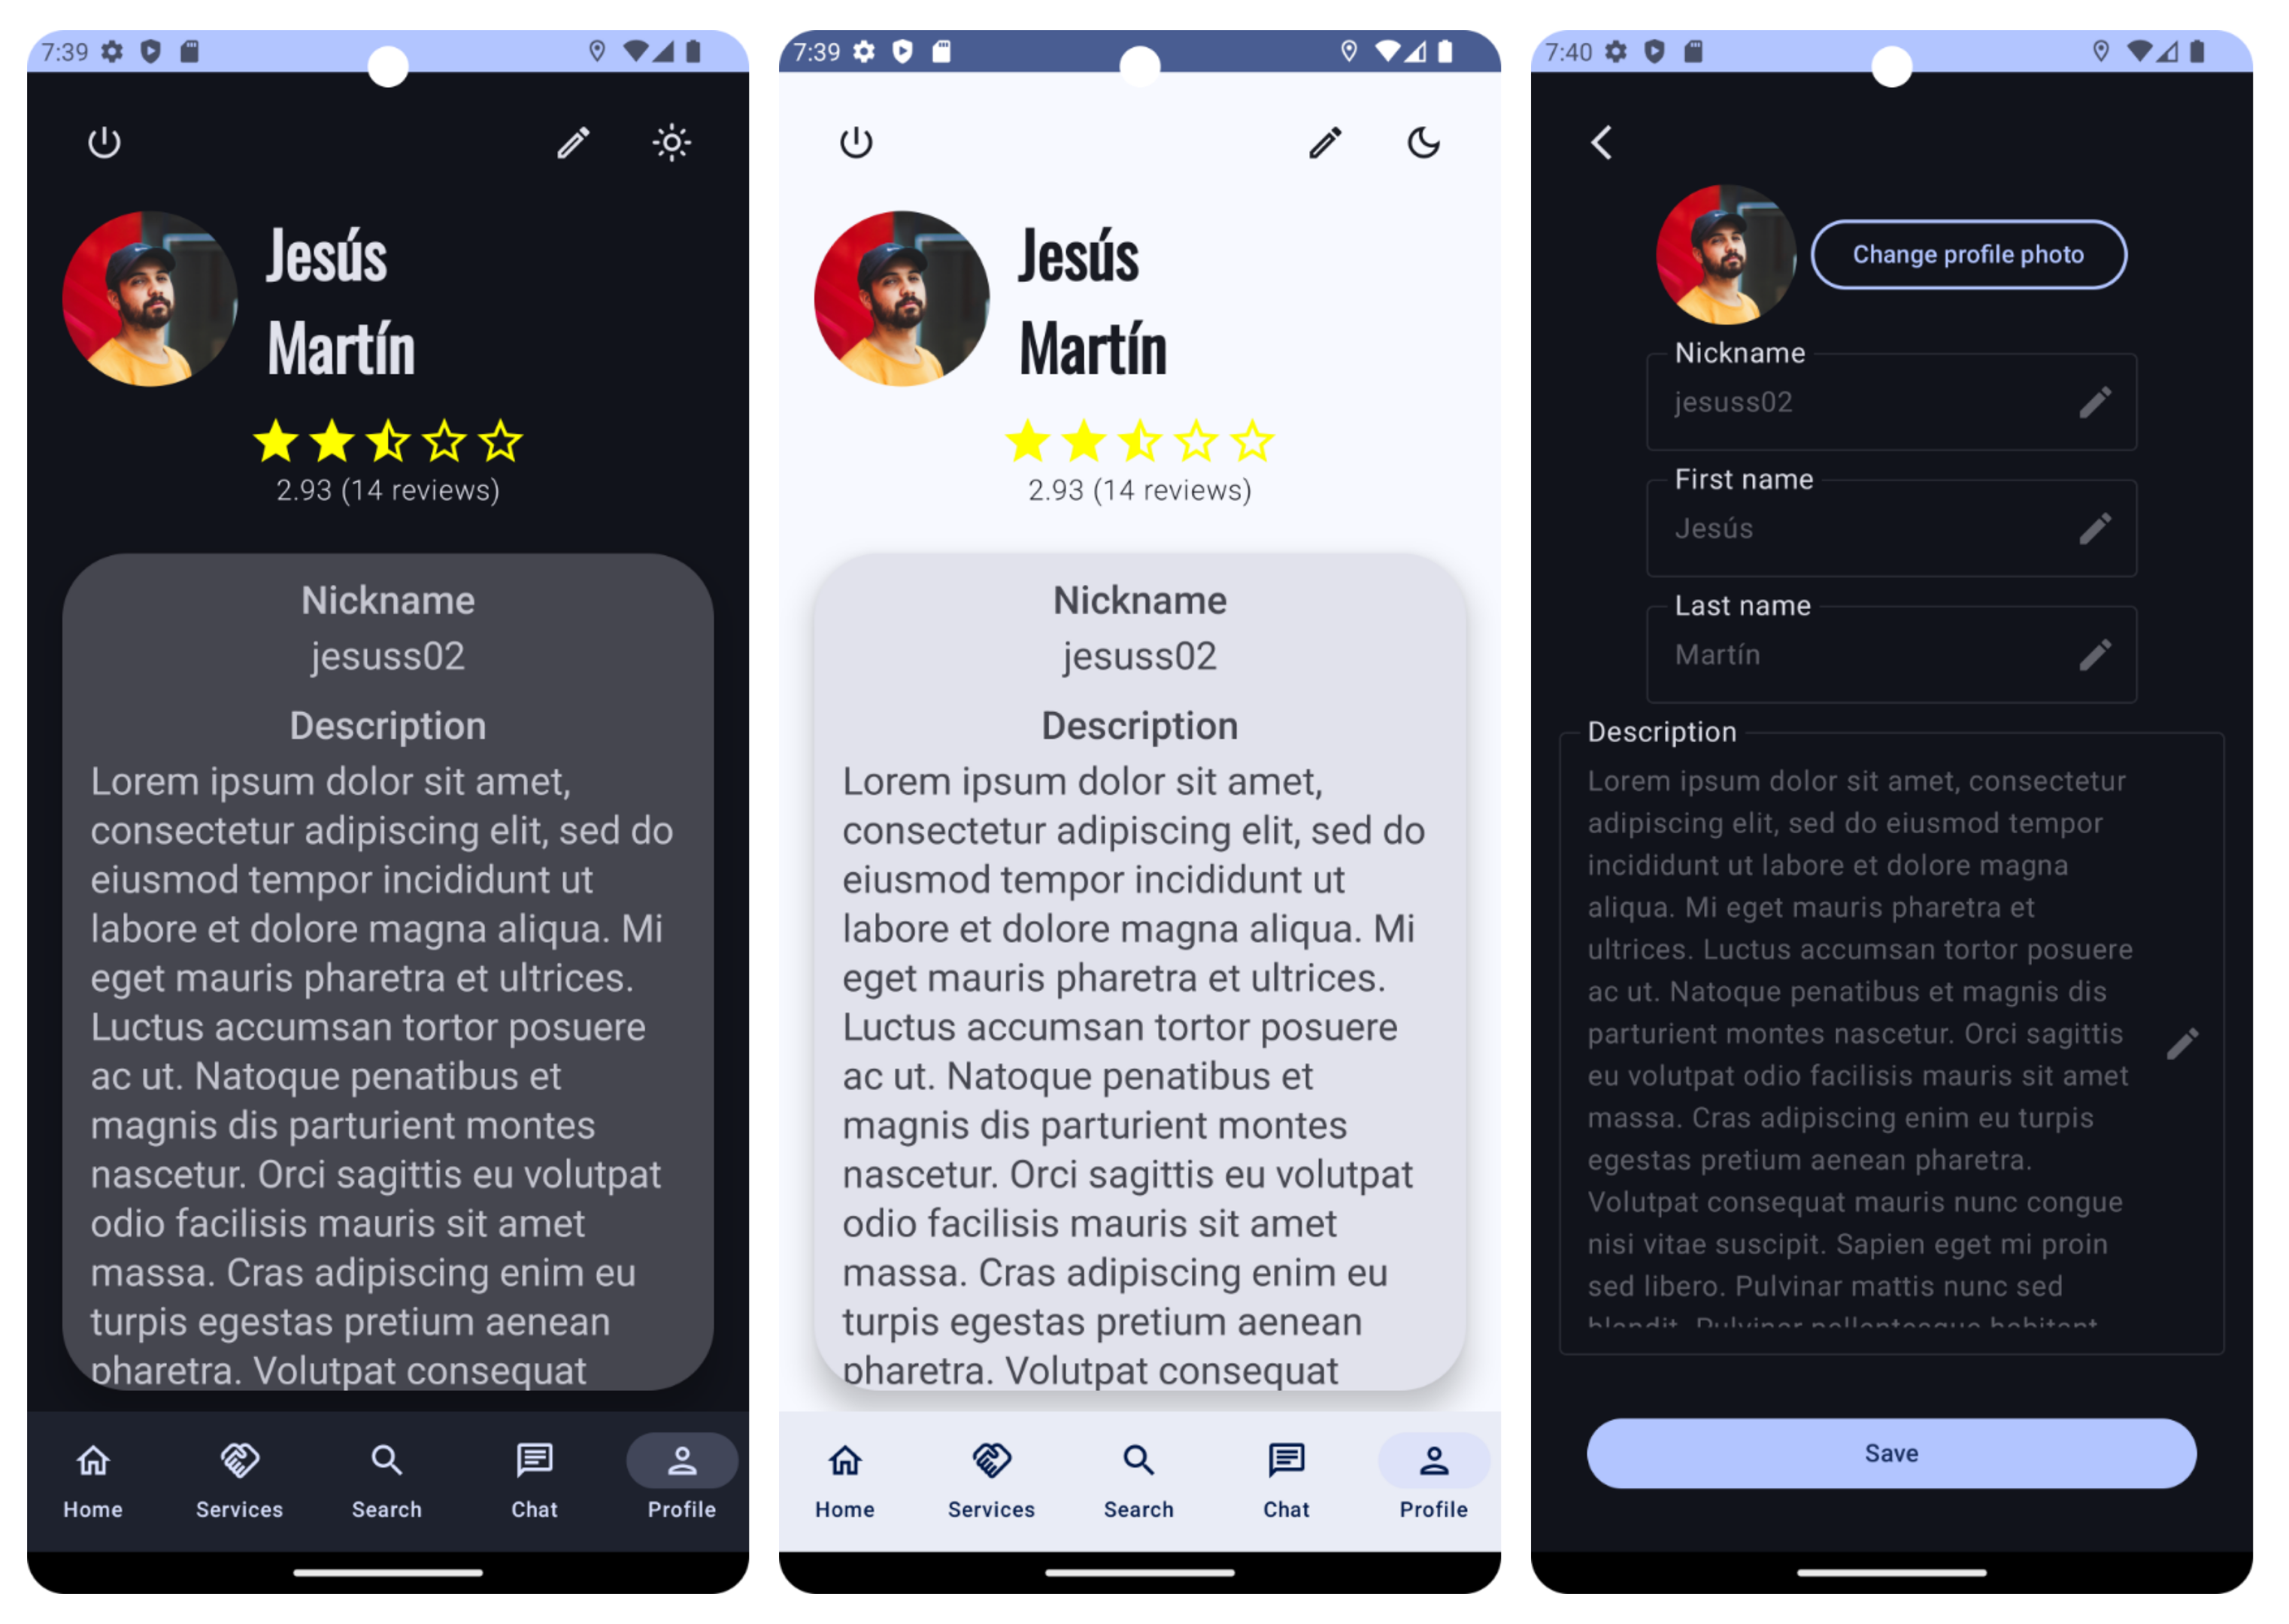
\includegraphics[width = 1\textwidth]{Imagenes/capturasApp/profile_light_edit.png}
	\caption{Profile Screen, Profile Screen (light), Edit profile Screen}
	\label{fig:capApp5}
\end{figure}

Por último, la sección del perfil propio es el último botón de la \textit{bottom bar} -captura 1, figura \ref{fig:capApp5}- en el se podrán ver todos los datos añadidos y la media de \textit{reviews}. Esta pantalla tiene también algunas funcionalidades extra como el cambio de tema de  la aplicación -ejemplo del modo claro en la captura 2, figura \ref{fig:capApp5}- y el \textit{logout} de la aplicación (icono de arriba a la izquierda). Pulsando el icono del lapiz se entra en la pantalla de edición del perfil -captura 3, figura \ref{fig:capApp5}-, en la que se podrá cambiar cualquier atributo del mismo, además de la foto de perfil, se podrá subir una foto de la galería o tomarla en el momento.

\section{Guía de profesional}
\label{sec:guiaProf}
